\subsection{Task 7: Triangle Counting}
According to the algorithms in \cite{tsourakakis2008fast}, we know that the number of triangles in a network is propotional to the sum of eigenvalue of its adjency matrix, which is $\frac{\sum_{i}\lambda_{i}^{3}}{6}$. Figure \ref{t7:timedata} shows the running time of global triangle counting with regards to the size of graph. We can see that as the size of graph increases, the running time also grows nearly linearly with the size. For the largest graph, which is Roadnet-PA, it runs nearly for an hour to complete. However, the predicted result for Roadnet-PA is unsatisfactory. We conduct both global and local triangle counting, all the data is listed as follows.

\subsubsection{Detailed Plots}
{\bf Proof of Correctness: } In this experiment, we run our algorithm on the dataset, and verify that the predicted number of triangles is a good approximate of the true count. The full result is in Table \ref{t7:globalpredict}. As we can see, most of the result is near to each other. So we are aure about the correctness of the implementation. 

Table \ref{t7:timedata} lists run time of global triangle counting. Figure \ref{t7:globaltime} plots the run time of global triangle counting on each dataset.

\begin{table}
\begin{center}
\begin{tabular}{ | c | c | }
    \hline
    graph size & run time(seconds) \\ \hline
    7115 & 45.199s \\ \hline
    36692 & 72.76 \\ \hline
    82168 & 596.046 \\ \hline
    334863 & 1288.703 \\ \hline
    1088092 & 2980.985 \\ \hline
\end{tabular}
\end{center}
\caption{Task 7 run time(global)}
\label{t7:timedata}
\end{table}

\begin{table}
\begin{center}
\begin{tabular} {| c | c | c | c | }
    \hline
    dataset & size & predict & truth \\ \hline
    wiki-Vite & 7115 & 661282 & 608389 \\ \hline
    Enron-email & 36692 & 756757 & 727044 \\ \hline
    slash-dot & 82168 & 635792 & 602592 \\ \hline
    Amazon-com & 334863 & 675778 & 667129 \\ \hline
    Roadnet-PA & 1088092 & 72134 & 67150 \\ \hline
\end{tabular}
\end{center}
\caption{Predicted triangle count(global)}
\label{t7:globalpredict}
\end{table}

% \begin{table}
% \begin{center}
% \begin{tabular} {| c | c | c | c | }
%     \hline
%     dataset & predict & truth \\ \hline
%     wiki-Vote & 661282 & 608389 \\ \hline
%     youtube & 3122234 & 3056386 \\ \hline
%     slashdot0922 & 631667 & 602592\\ \hline
%     com-DBLP & 2451225 & 2224385 \\ \hline
%     wiki-Talk & 9778534 & 9203519\\ \hline
% \end{tabular}
% \end{center}
% \caption{Predicted triangle count(global)}
% \label{t7:globalpredict}
% \end{table}

\begin{figure}[!htbf]
\begin{center}
\begin{tabular}{c}
     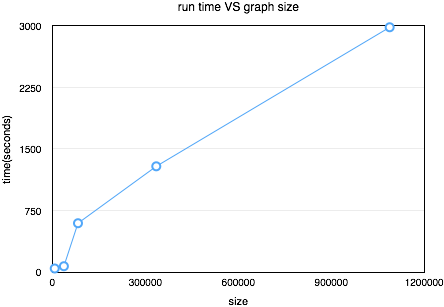
\includegraphics[width=0.6\textwidth]{FIG/t7_time.png}
\end{tabular}
\caption{Task 7: Run time VS graph size(global)}
\label{t7:globaltime}
\end{center}
\end{figure}

\subsubsection{Local triangle counting}
We plot the rank-frequency plot of local triangle counting, that x-axis represent the rank of the count of local triangle, y-axis represents the number of local triangles at that rank. 

\paragraph{Amazon}
Figure \ref{t7:amazon} plots the rank-frquency of Amazon. We can observe from the figure that it follows {\bf power law}. 
\begin{figure}[!htbf]
\begin{center}
\begin{tabular}{c}
     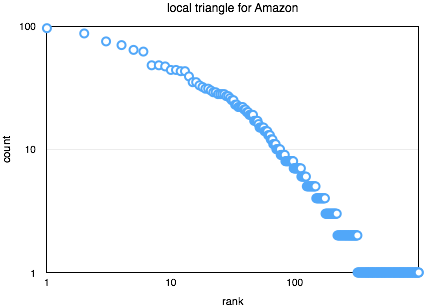
\includegraphics[width=0.4\textwidth]{FIG/t7_amazon.png}
\end{tabular}
\caption{Local triangle counting for Amazon}
\label{t7:amazon}
\end{center}
\end{figure}

\paragraph{Enron mail}
Figure \ref{t7:enron} plots the rank-frquency of Enron Mail. We can observe from the figure that it follows {\bf power law}. 
\begin{figure}[!htbf]
\begin{center}
\begin{tabular}{c}
     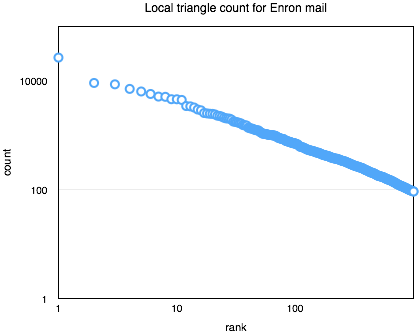
\includegraphics[width=0.4\textwidth]{FIG/t7_enron.png}
\end{tabular}
\caption{Local triangle counting for Enron mail}
\label{t7:enron}
\end{center}
\end{figure}

\paragraph{Slashdot}
Figure \ref{t7:slashdot} plots the rank-frquency of Slashdot. We can observe from the figure that it follows {\bf power law}. 
\begin{figure}[!htbf]
\begin{center}
\begin{tabular}{c}
     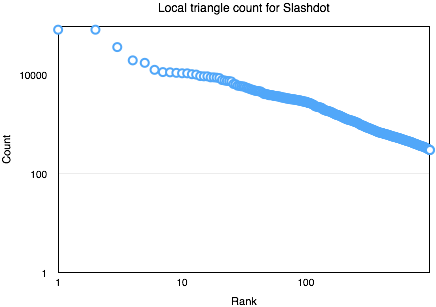
\includegraphics[width=0.4\textwidth]{FIG/t7_slashdot.png}
\end{tabular}
\caption{Local triangle counting for Slashdot}
\label{t7:slashdot}
\end{center}
\end{figure}

\paragraph{wiki-Vote}
Figure \ref{t7:wikivote} plots the rank-frquency of wiki-Vote. We can observe from the figure that it follows {\bf power law}. 
\begin{figure}[!htbf]
\begin{center}
\begin{tabular}{c}
     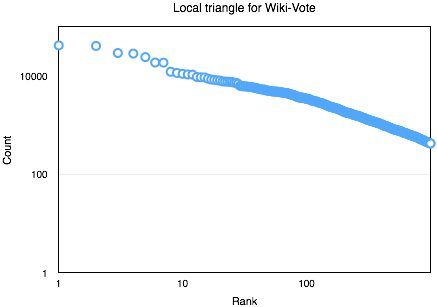
\includegraphics[width=0.4\textwidth]{FIG/t7_wikivote.png}
\end{tabular}
\caption{Local triangle counting for wiki-Vote}
\label{t7:wikivote}
\end{center}
\end{figure}

\paragraph{Youtube}
Figure \ref{t7:youtube} plots the rank-frquency of Youtube. We can observe from the figure that it follows {\bf power law}. 
\begin{figure}[!htbf]
\begin{center}
\begin{tabular}{c}
     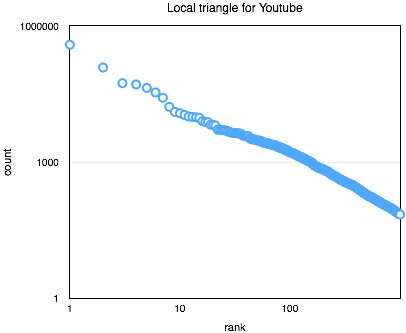
\includegraphics[width=0.4\textwidth]{FIG/t7_youtube.png}
\end{tabular}
\caption{Local triangle counting for youtube}
\label{t7:youtube}
\end{center}
\end{figure}

% \begin{figure}[!htbf]
% \begin{center}
% \begin{tabular}{cc}
%      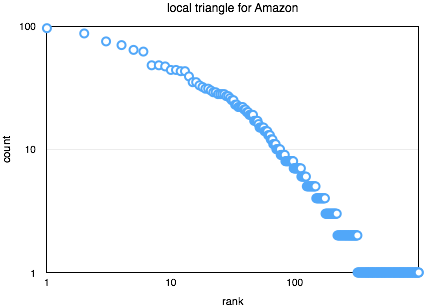
\includegraphics[width=0.4\textwidth]{FIG/t7_amazon.png} &
%      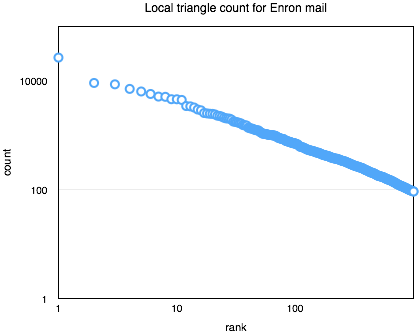
\includegraphics[width=0.4\textwidth]{FIG/t7_enron.png} \\
%      (a) & (b) \\
%      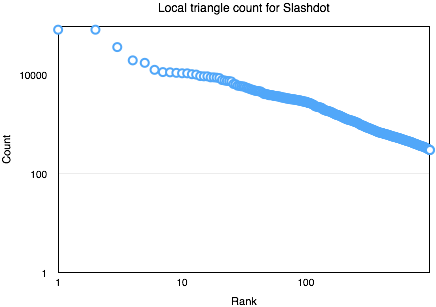
\includegraphics[width=0.4\textwidth]{FIG/t7_slashdot.png} &
%      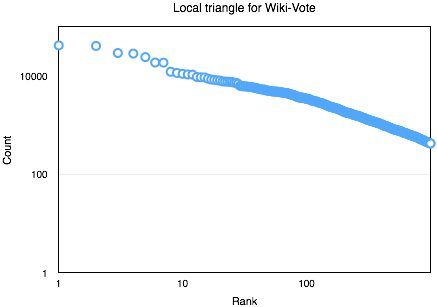
\includegraphics[width=0.4\textwidth]{FIG/t7_wikivote.png} \\
%      (c) & (d) \\
%      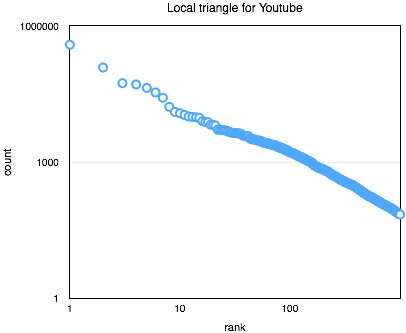
\includegraphics[width=0.4\textwidth]{FIG/t7_youtube.png} & \\
%      (e)
% \end{tabular}
% \caption{Local triangle counting. (a) Amazon (b) Enron Mail (c) Slashdot (d) Wiki Vote (e) Youtube}
% \label{t7:local}
% \end{center}
% \end{figure}

\subsubsection{Observation}
We can see that the rank-frequency plot of local triangle count also follows {\bf power law}, it just matches our intuition. And we can observe that the run time grows nearly linearly with the graph size. 
